\documentclass{beamer}
\usepackage{subcaption}
\usepackage{tikz}
\usepackage[numbers, authoryear]{natbib}





\title{Deep Reinforcement Learning for an NP-Hard Scheduling Problem}
\author{Elisabeth Bankl, BSc}
\institute{FH Technikum Wien}
\date{\today}

\begin{document}

\begin{frame}
    \titlepage
    \vspace{-1cm} % Adjust spacing if needed
    \begin{center}
        \usebeamerfont{author}Supervisor: Dipl.-Ing. Dipl.-Ing. Dr. techn. Christoph Redl, BSc
    \end{center}
\end{frame}


\begin{frame}
    \frametitle{Research Questions}
    \begin{itemize}
\item How effectively can a scheduling problem be solved using Deep Reinforcement
 Learning?
 \item How close to optimal are the solutions the RL agent discovers, in percentage,
 depending on problem size?
 \item Can the RL agent compete with state-of-the-art solutions in terms of
 execution time and achieved optimality?
\end{itemize}
\end{frame}

\begin{frame}
    \frametitle{Problem Statement}
    \begin{itemize}
        \item Tasks need to be completed sequentially
        \item Some tasks must be finished before starting others (precedence constraints)
        \item The execution time of a task depends on the task before it (transition time)
        \item Goal: Order the tasks in a way that minimizes the total execution time and follows all precedence constraints
        \item Sequential Ordering Problem (SOP) / Asymmetric Travelling Salesperson Problem with Precedence Constraints

    \end{itemize}
\end{frame}


\begin{frame}
    \frametitle{Graph Representation}
    \begin{figure}[H]
        \centering
        \begin{subfigure}[b]{0.45\textwidth}
            \centering
            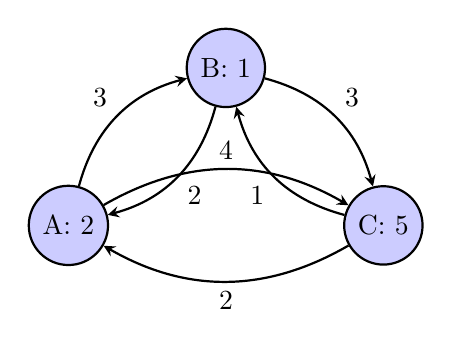
\begin{tikzpicture}[->, >=stealth, auto, thick, node distance=2cm]
                \node[circle, draw, fill=blue!20] (A) at (0,0) {A: 2};
                \node[circle, draw, fill=blue!20] (B) at (2,2) {B: 1};
                \node[circle, draw, fill=blue!20] (C) at (4,0) {C: 5};

                \draw[->] (A) to[bend left] node {3} (B);
                \draw[->] (A) to[bend left] node {4} (C);
                \draw[->] (B) to[bend left] node {2} (A);
                \draw[->] (B) to[bend left] node {3} (C);
                \draw[->] (C) to[bend left] node {2} (A);
                \draw[->] (C) to[bend left] node {1} (B);
            \end{tikzpicture}
            \caption{Distances}
        \end{subfigure}
        \hfill
        \begin{subfigure}[b]{0.45\textwidth}
            \centering
            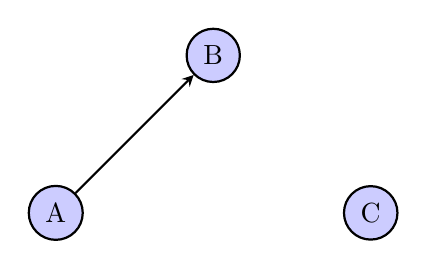
\begin{tikzpicture}[->, >=stealth, auto, thick, node distance=2cm]
                % Define nodes
                \node[circle, draw, fill=blue!20] (A) at (0,0) {A};
                \node[circle, draw, fill=blue!20] (B) at (2,2) {B};
                \node[circle, draw, fill=blue!20] (C) at (4,0) {C};

                % Draw a single directed edge with a weight
                \draw[->] (A) to node {} (B);
            \end{tikzpicture}
            \caption{Precedence constraints}
        \end{subfigure}
    \end{figure}
\end{frame}


\begin{frame}
    \frametitle{Formal Problem Definition (1/2)}

    Adapted from \cite{schoen2024optimization}.

    
    Let \( V = \{1, 2, \ldots, n\} \) be the set of nodes.
    
    \( c_i \): cost for visiting node \( i \) first
    
    \( c_{ij} \): cost for moving from node \( i \) to node \( j \)
    
    Precedence constraints: if \( p_{ij} = 1 \), node \( i \) must be visited before node \( j \).

    
    Binary variable \( y_i \) for \( i \in V \) as:
    \[
    y_i = 
    \begin{cases} 
    1 & \text{if node } i \text{ is the first node in the tour} \\ 
    0 & \text{otherwise}
    \end{cases}
    \]
    The sum of these variables should be 1:
    \[
    \sum_{i \in V} y_i = 1
    \]
\end{frame}

\begin{frame}
    \frametitle{Formal Problem Definition (2/2)}
    
    Binary variable \( y_{ij} \) for \( i \in V \) and \( j \in V \setminus \{i\} \) as:
    \[
    y_{ij} = 
    \begin{cases} 
    1 & \text{if the tour includes the edge} (i,j) \\ 
    0 & \text{otherwise}
    \end{cases}
    \]
    \[
        0 \leq \sum_{j \in V \setminus \{i\}}  y_{ij} \leq 1
    \]
    
    \[
    \sum_{i \in V \setminus \{j\}} y_{ij} + y_j = 1
    \]
    
    Objective: Minimize the total cost of the tour:
    \[
    \min  \sum_ {i \in V} c_i y_i + \sum_ {i \in V} \sum_{j \in V \setminus \{i\}} c_{ij} y_{ij}
    \]
\end{frame}



\begin{frame}
\frametitle{Existing algorithms}

\begin{itemize}
\item \textbf{Greedy / Nearest Neighbor Algorithm}

Iteratively go to the nearest unvisited node \cite{atsp}
\item \textbf{LKH-3} 

A variable-depth local search heuristic \cite{lkh3}.
\item \textbf{Branch and Bound}

Uses the dynamic Hungarian algorithm to find lower bounds and a local-search domination technique to prune suboptimal branches
\cite{branch_bound_sop}

\item \textbf{Ant Colony Optimization}

A metaheuristic where artificial ants deposit pheromones on selected edges to guide optimization  \cite{antcolony}
\end{itemize}
\end{frame}


\begin{frame}
    \frametitle{Markov Decision Process}
    \begin{itemize}
        \item \textbf{State Space}: 
        \begin{itemize}
            \item \textbf{Distance Matrix (D)}: Distances between nodes
            \item \textbf{Precedence Matrix (P)}: Which nodes must be visited before others
            \item \textbf{Cost Matrix (C)}: Cost of choosing a node as the first node in the tour, later cost for choosing a node next
            \item \textbf{Visited Nodes Matrix (V)}: A binary matrix indicating which nodes have been visited.
        \end{itemize}
        \item \textbf{Action Space}: The actions are the nodes that the agent can visit next.
        \begin{itemize}
            \item Nodes with unmet precedence constraints are not allowed.
            \item Previously visited nodes are not allowed.
        \end{itemize}
        
    \end{itemize}
\end{frame}

\begin{frame}
    \frametitle{Reinforcement Learning Algorithm}
    \begin{itemize}
        \item \textbf{Reward}:
        \begin{itemize}
        \item Negative cost of selecting the first node in the path
        \item Negative distance between nodes
        \end{itemize}
        \item \textbf{Algorithm}: Maskable Proximal Policy Optimization (PPO) \cite{schulman2017proximalpolicyoptimizationalgorithms}
        \item \textbf{Network Architecture}: MLP
    \end{itemize}
\end{frame}

\begin{frame}
    \frametitle{Dataset}
    \begin{itemize}
        \item Available datasets for SOP:
        \begin{itemize}
        \item Not enough instances for training
        \item Used for benchmarking
        \end{itemize}
        \item Randomly generate problem instances during training. 
        \begin{itemize}
        \item Distances between nodes are sampled from a uniform distribution
        \item Precedence constraints are sampled from binary distribution with probability p
        \item Node costs from a uniform distribution
        \end{itemize}
        \item Distances between the nodes follow the triangle inequality $c_{ij} + c_{jk} \geq c_{ik}$
        \item Size: 25 nodes
        
    \end{itemize}
\end{frame}


\begin{frame}
    \frametitle{Performance Evaluation}
    \begin{figure}
        \centering
        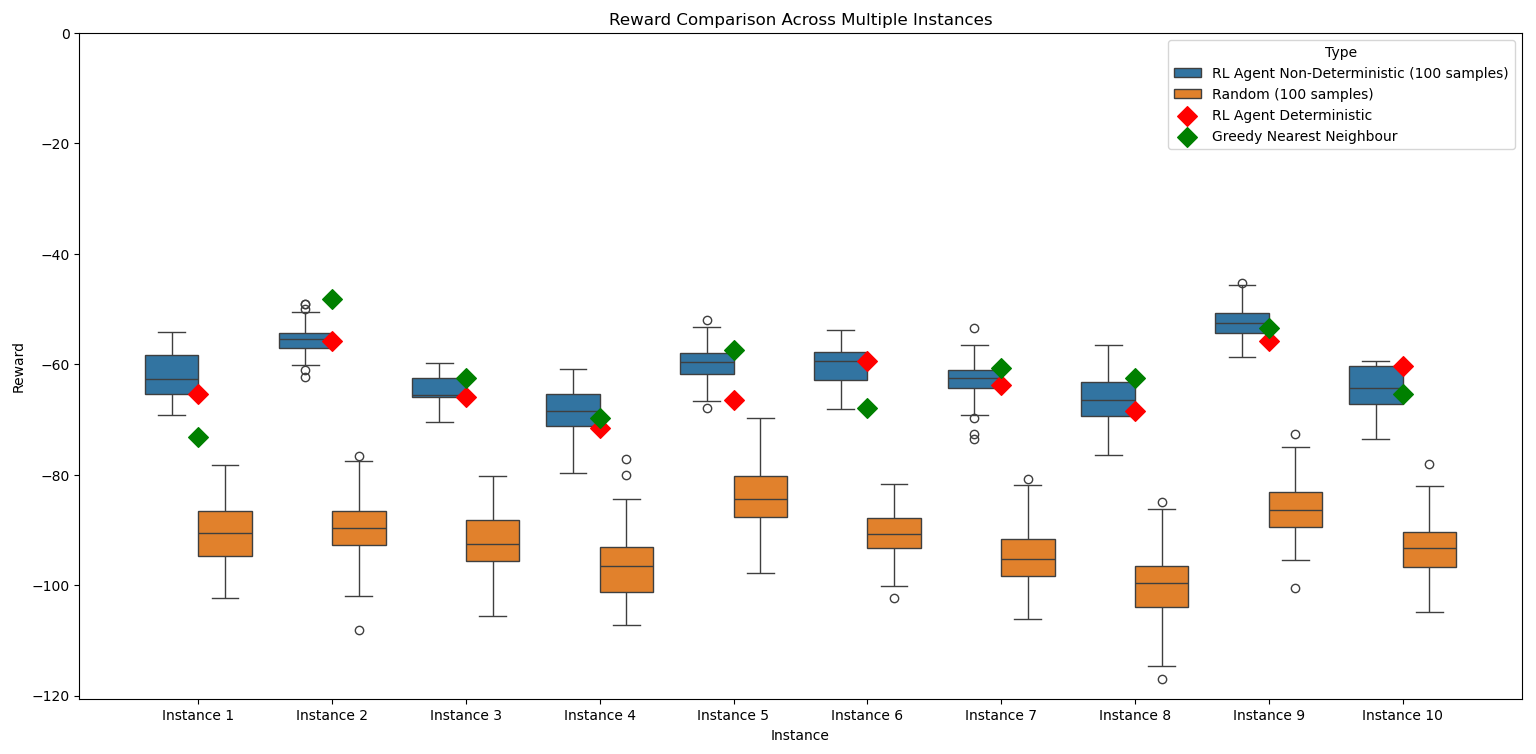
\includegraphics[width=1\textwidth]{10_instances_new.png}
        \caption{Comparing of the average reward of the agent with the simple greedy heuristic and random paths (p = 0.1).}
    \end{figure}
\end{frame}

\begin{frame}
    \frametitle{Performance Evaluation depending on the precedence constraints}
    \begin{figure}
        \centering
        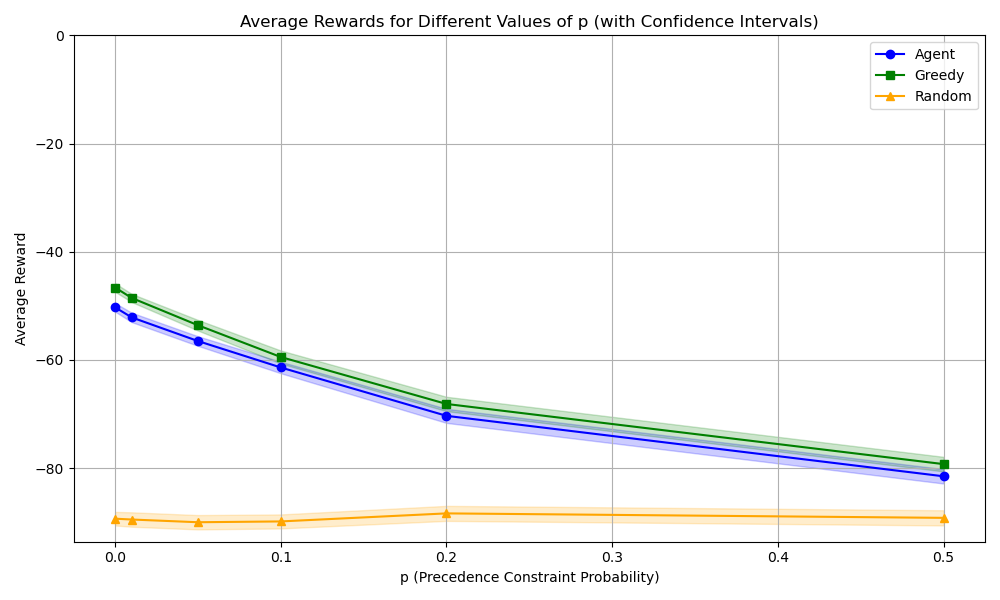
\includegraphics[width=1\textwidth]{average_reward_over_p.png}
        \caption{Comparing the average reward achieved by the agent, the simple greedy heuristic and random paths.}
    \end{figure}
\end{frame}



\begin{frame}
\frametitle{Current Limitations \& Next Steps}
\begin{itemize}
    \item Maximum problem size: 25 nodes
    \item The RL agent's performance is still worse, on average, than the greedy heuristic.
    \item Change the problem instances
    \begin{itemize}
        \item Make instance generator more deterministic
        \item Clustered instances
        \item Use existing instance generators
    \end{itemize}

\item Experiment with different RL algorithms
\begin{itemize}
    \item Deep Q-Learning and its variants
\end{itemize}
\item Reward Shaping: use $\frac{1}{r}$ or $-r^2$ instead of $-r$

\item Modify network Architecture:
\begin{itemize}
\item GNN
\item Attention
\end{itemize}


\end{itemize}

\end{frame}
 
\begin{frame}[allowframebreaks]
    \frametitle{References}
    \bibliographystyle{apalike}
    \bibliography{references}
\end{frame}


\end{document}